\section{Evaluation of Environmental Wireless Sensor Networks (E-WSN)}
\label{section:experimental}	
\begin{figure}[ht]
	\centering
	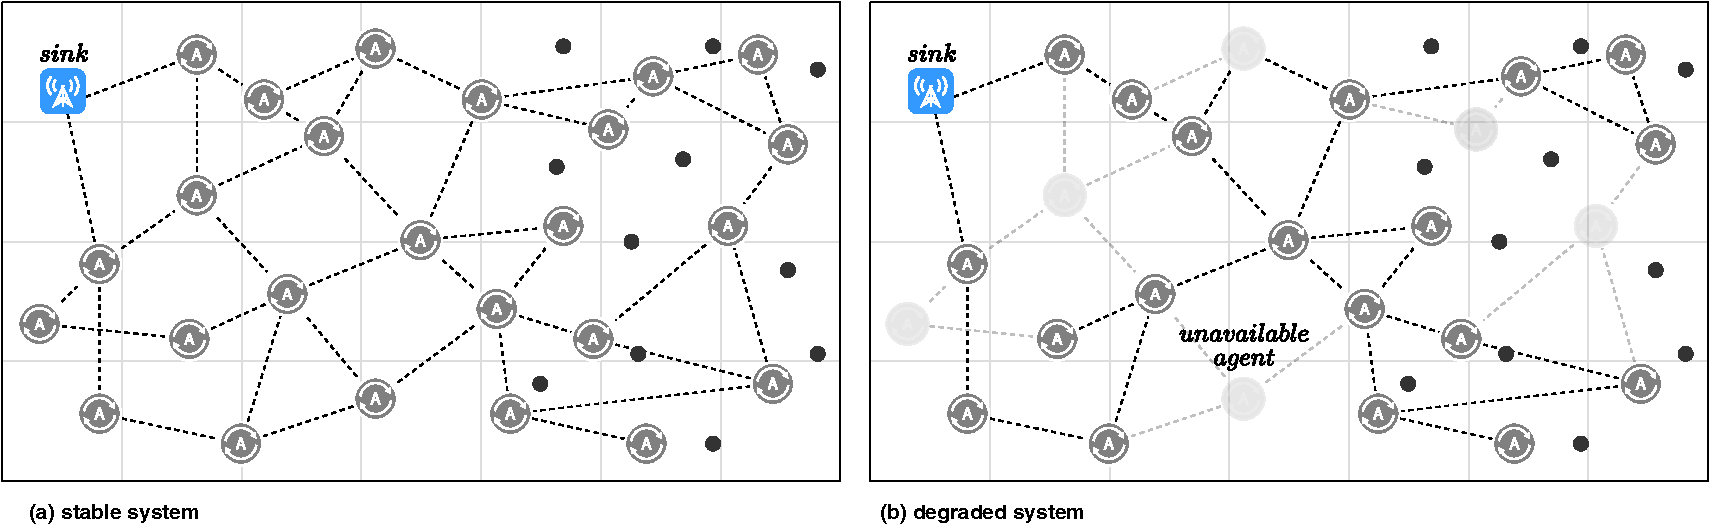
\includegraphics[width=0.9\linewidth, trim={25pt 0pt 25pt 0pt, clip}]{system-types}
	\caption{\textbf{System types}. The diagram shows examples of the two systems. In the first \simulationSimple{}{}, there are $10$ possible agents that can execute the measurement task, tasks' demand points are distributed across the map. In the second, \simulationExtended{}{} system, there are $25$ agents that can execute the measurement tasks. The tasks' demand points are clustered away from the sink node.}
	\label{fig:system-types}
\end{figure}
\begin{figure}[ht]
	\centering
	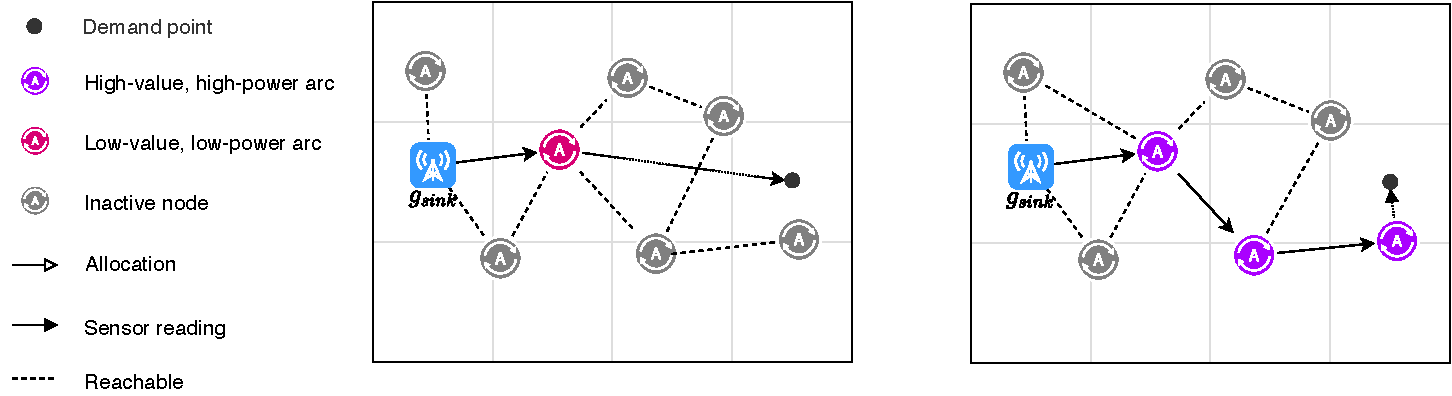
\includegraphics[width=0.9\linewidth, trim={25pt 0pt 25pt 0pt, clip}]{route-types}
	\caption{\textbf{Routes, power consumption, and task value}. The diagram shows two possible task-paths for the same system. In the first, energy is conserved by having a short task-path but the task is completed to a lesser quality. In the second, the maximum quality for the task is achieved, however, there is more energy consumption overall.}
	\label{fig:route_types}
\end{figure}

The simulation framework to evaluate the algorithms' performance was based on a realistic deployment scenario as covered by  \cite{Gomez2015} and others \citep{Jha2016, Avram}. In this scenario a UAV is used to deploy a large number of sensors over a expansive and remote geographical area, giving an ad-hoc, randomised placement of devices. Solar power cells are used to maintain enough energy to power the sensors over a number of years, given low enough power consumption. We simulated two systems and evaluated the algorithm in four different configurations (See Figure \ref{fig:system-types}).  The simple system simulates a standard environment and is focused on the examination of energy and quality optimisation. The extended system is structured to test the algorithms' performance in task-path selection given different configurations.  As a baseline we use the \acronymQRouting{}{} algorithm, which uses state-of-the-art Q-learning techniques to optimise network routes based on energy consumption and task quality equally \citep{XXX, XXX}.

The \simulationSimple{}{} system  equal weighting for each of the CTV components $\alpha, \beta, \gamma$ (Eq. \ref{eq:ctv}). The sink node was given $5$ measurement tasks to complete from outside the system. The tasks were repeated $3$ times before one episode was complete to highlight the increase the energy demands on the system. $10$ nodes were distributed randomly in the system, each one initially connected to $3$ other nodes that were randomly chosen with a bias towards closer located nodes\footnote{
	The probability of initial node selection used the standard gamma distribution $f(x; \alpha, \beta) = \frac{\beta^{\alpha} x^{\alpha-1}e^{- \beta x}}   {\Gamma(\alpha)}$, where $\Gamma(\alpha)$ is the  gamma function, $\alpha=1.8, \beta=0.5$, and $x$ is the unit distance between the two nodes.
}.  Each node was capable of completing a task, or allocating it to any of $3$ nodes it was connected to. They could complete any measurement task with a quality dependent on their closeness to the demand point associated with the task (Eq. \ref{eq:atomic_task_quality}). The energy of all nodes in the system was fully reset at the end of each episode. An example of the simple system layout can be seen in Figure \ref{fig:system-types}(a). 
